\documentclass[UTF8]{ctexart}
\usepackage{amsmath}
\usepackage{forest}
\usepackage{algorithm}
\usepackage{algorithmic}
\usepackage{tabularx}
\usepackage{booktabs}
\usepackage{enumerate}
\title{\vspace{-4cm}2023体系结构读书报告}
\author{2000013058 杨仕博}
\date{\today}
\begin{document}
\maketitle

\section{报告摘要}

\subsection{DEFINITIONS}

本节旨在给高速自动电子计算系统一个一般性的解释说明。
自动计算系统被定义为一个可以执行指令以完成相当复杂计
算的设备——指令需要提供相当详尽的数值细节,并通过某种
设备可以感知的方式给出;而设备需要在不给出人类智能干
预的情况下运行这些指令,并以某种形式输出结果。为得到
结果,这个设备可能产生诸多中间值,他们循环在设备内部
,不会被输出以被人类感知。

作为一个复杂的系统,该设备
与他的长序列操作将不可避免地存在存在故障的可能性,这
种故障将影响设备的输出——然而,我们可以在某种程度上避
免之,譬如令设备识别常见错误,以某种形式定位并输出故
障,甚至自动改正故障并做出正确行动。

\subsection{MAIN SUBDIVISIONS OF THE SYSTEM}

在分析这个复杂的设备时,系统的某些必须的、互不相同的组件
就需要被立即划分出来。

\paragraph{CA}

为实现计算,基本的运算操作应当需要被实现。尽管具体
实现哪些运算是未定的、以何种方式实现之也是未定的,但这种运算
模块是系统中必然存在的部分,我们称此为CA。

\paragraph{CC}

为赋予计算设备实现近乎全部算法的能力,将有限的指令集与一个能够
基于它们摆放出合适运算序列的控制模块分离开来就是必要的设计了——
这就是控制器CC。

\paragraph{M}

执行长且复杂的机器必然需要足够大的内存空间,以在足够复杂的计算
目标下存储中间结果、间接逻辑生成的材料、必要的表、问题设定的
特定的条件等等。

\paragraph{R}

信息最原始的来源和最后输出时的目标均为人类可写入或感知的外部,
我们需要一种可以和C、M交互的介质存储这些信息——我们把它记为R。

\paragraph{IO}

由上,我们分别需要一些机制来将R中的信息传向C、M,或者将C与M中
的信息传向R——因而,我们需要输入输出设备I、O。

事实上,R同样具有记忆的属性,他同样具备M的功能。在功能上二者的区别
主要在于M相对更快一些——但适当地混用二者不会造成速度上过多的
损耗,同时可以同时处理更大量的数据。

\subsection{PROCEDURE OF DISCUSSION}

这一章旨在指明如何逐步讨论出五个模块的功能。我们希望讨论出每部分
各自的特点、相互的联系,以及这个机器处理问题的具体逻辑。
但是,完全抛弃其余部分地讨论完一个
部分不甚现实,因而我们需要各部分互相穿插地逐步刻画所出有模块的逻辑,
结合实际地在最终凝结出我们所需要的设计图。

特别地,作者指出,对于自动纠错
这种问题,虽然我们未必可以完全清楚地讨论它,但至少也需要给予它一些粗浅的考量。

\subsection{ELEMENTS, SYNCHRONISM, NEURON ANALOGY}

\paragraph*{ELEMENTS}

所谓元素是可以维持信息的元件,他以某种方式永久地维持某状态,
并通过特定的刺激改变状态——这种状态可以传递,并且与能量无关(不
随传递而丧失状态)。这种物理器件在现实中是可以实现的。

这些元素可以自动“计时”,或是通过自身,或是通过一个固定的时钟
刺激。其区别在于后者可以完成元素间的同步,而我们也以此划分设备
是同步设备亦或异步设备。

而生物的神经元正是具备这种维持状态能力的天然器件,他们可以维持
状态,并不类似能量一样地传播。同时,神经元之间的交互也存在延迟。

同时,作者指出真空管元件具有极快的速度,是构建元素的合适之选;
而且,同步设备较异步更优。

\subsection{PRINCIPLES GOVERNING THE ARITHMETICAL OPERATIONS}

现有器件中天然地维持着两个平衡态,而更多的平衡态将导致更多的问题,
这指明这一计算系统更适合于使用二进制体制。人类神经元亦为二元。

二进制大大减轻了计算的复杂度,因而在CA和CC以及M中应该使用二进制。
然而人类更适合与十进制交互,因而R中的存储应该是十进制的。这就要
求IO具备进制转换功能。为方便计算和协调,这里同样需要CC和CA。

二进制带来的问题是逐比特运算次数过多。然而,十进制的少数运算
需要以昂贵的乘法表作为代价。这个代价下二进制运算也能得到优化,
因而不单独讨论十进制是合适的。

二进制巨量的、不可接受的运行次数可以由并行运算解决。也即通过
等倍数增加运算电路的量配合适当的、同时多比特运算的算法以换得
相应的速度。
由于时间对于机器至关重要,因而这是合理的。

不同物理原件、不同运算的速度又招致了保持同步的问题。但是对不同
器件具体速度的不确定又不好让我们决定如何加速算术运算。同样,
真空管的并行也会另其效率降低——这又让我们希望尽量简化设备和并行。

而是否需要完全简化并行以简化设备需要与物理元件妥协。所以,最终
需要两种方向博弈地思考。

\subsection{E-ELEMENTS}

进一步讨论需要基于元件的基本功能之上,而如果详细剖析则会陷入
元件工程上的细节中。因而,我们需要对元件功能进行抽象,在必要时
再重新返回元件更底层的设计中。

人类的神经元就是一个很好的抽象模型。我们认为所有神经元只具有
同样且一定的突触延时$\tau$(这在电路上是合理的)。这个时间可以
作为时间单位来完成我们的同步,具体来说,是通过合理安排时钟的
脉冲刺激时间来完成同步。

在本章的抽象中,一个E-ELEMENT可以接受兴奋性突触或抑制性
突触的信号传递,并根据兴奋性突触的刺激数决定状态的转变。其延时
是$\tau$的整数倍。

平均而言,每个E-ELEMENT越由两个真空管组成。

\subsection{CIRCUITS FOR THE ARITHMETICAL OPERATIONS +, ×}

为简化设备,文中选择将一个30位的数字由30$\tau$时间内的30次刺激
的存在性表示。成套的组件将被包装为一个块。

文中同样使用比特加和同位的结果与进位合并的方式完成了1bit加法器
的构建。

而乘法器需要对每一bit都进行多次运算,不可能如加法器一般直接
输出结果,因而它需要有存储功能的器件。为方便,我们没有使用M,
而是在CA中开辟额外的存储空间。

E-ELEMENT可以输出通向自身+set/reset功能完成1bit存储。
通过多个如此的存储或者多个E-ELEMENTS循环可以得到多bit存储。
同时,简单的线性串联也可以延迟地存储信息,但是也有非E-ELEMENTS
的器件可以替换之,我们也将此视为一种元件。

有了这些我们就可以实现乘法器。通过定时输出刺激的器件+通过输入
和刺激判断是否要发送对应刺激的器件就可以完成乘法中按乘数的
0/1决定是否把被乘数放入加法器的功能,进而完成乘法,而这两个
器件可以通过多个需要2输入改变状态的元件组合和dl(延时器)而成。

这里的延时器也将不可避免一些同步的问题,但是一些取舍和调整即可
处理好这些。同时,符号和二进制点的位置这类问题也是需要在之后
解决的。

\begin{figure}[H]
\centering
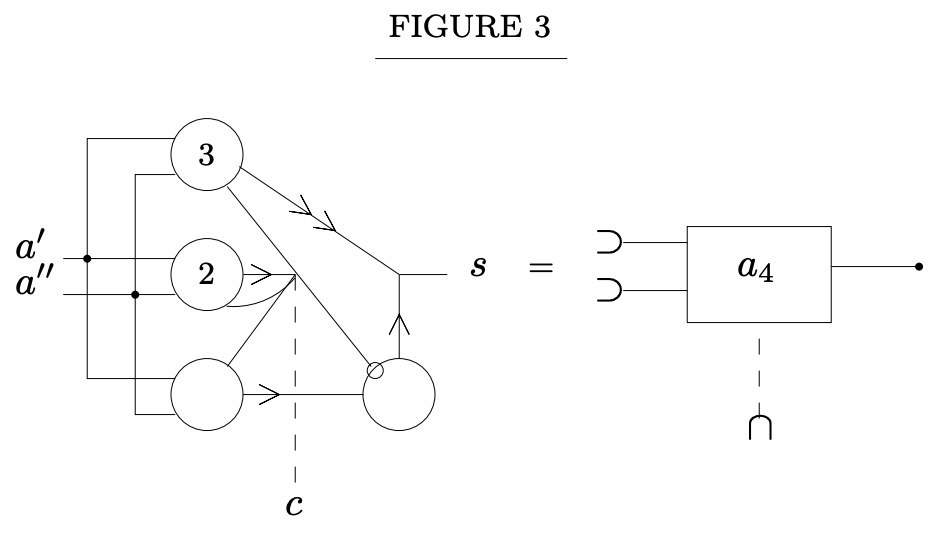
\includegraphics[width=\textwidth]{./pics/9.jpeg}
\caption{加法器}
\end{figure}

\begin{figure}[H]
\centering
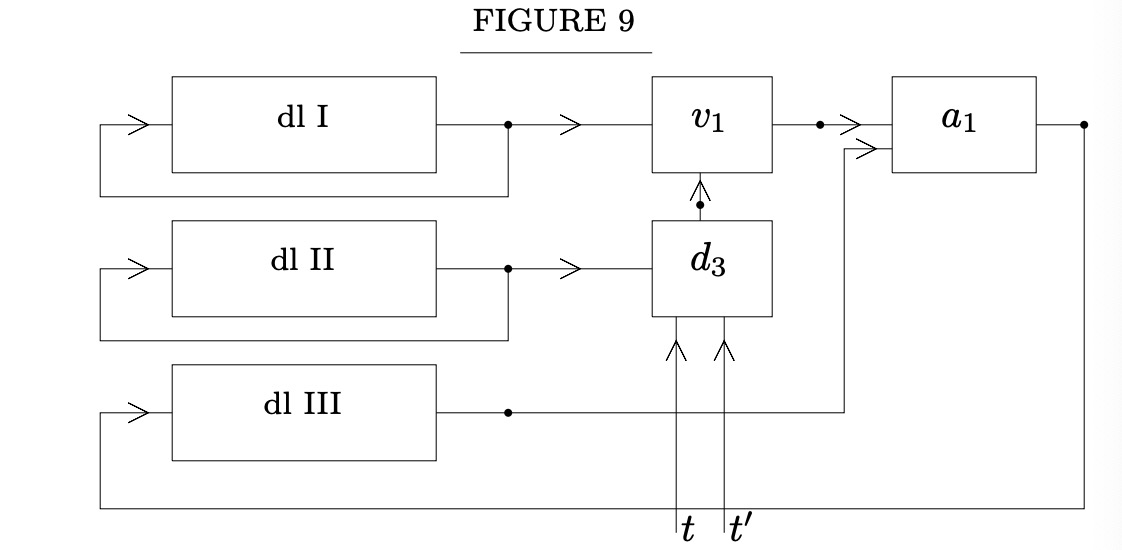
\includegraphics[width=\textwidth]{./pics/10.jpeg}
\caption{乘法器}
\end{figure}

\subsection{CIRCUITS FOR THE ARITHMETICAL OPERATIONS −, ÷}

为定义减法,我们按照补码的方式定义负数。这使加法兼容了减法——
只需要在加法器上配套补码计算器即得到了减法器。

除法的逻辑是每次判断除数减现在的余数是否为负以确定商对应位
是否为1——这个判断逻辑相比乘法更为复杂,但是通过更复杂的、
由我们之前所提到的元件的排列仍然可以完成这个需求,进而组件出
除法器。

相应的,除法器也在定时网络、延迟长度、符号和二进制点的问题上
有类似于乘法的问题需要在以后解决。

\begin{figure}[H]
\centering
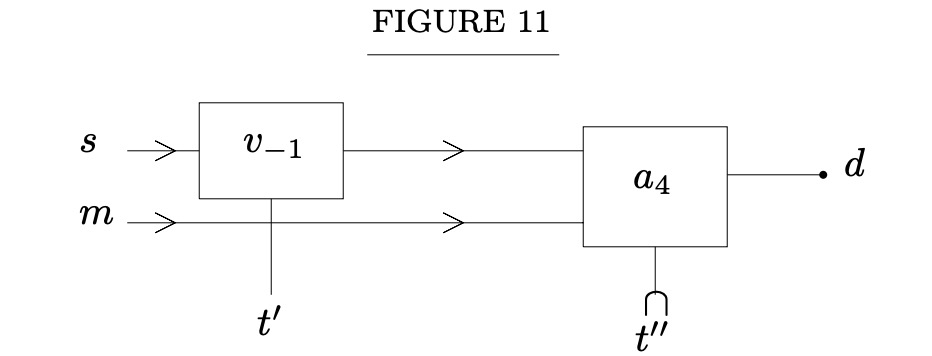
\includegraphics[width=\textwidth]{./pics/11.jpeg}
\caption{减法器}
\end{figure}

\begin{figure}[H]
\centering
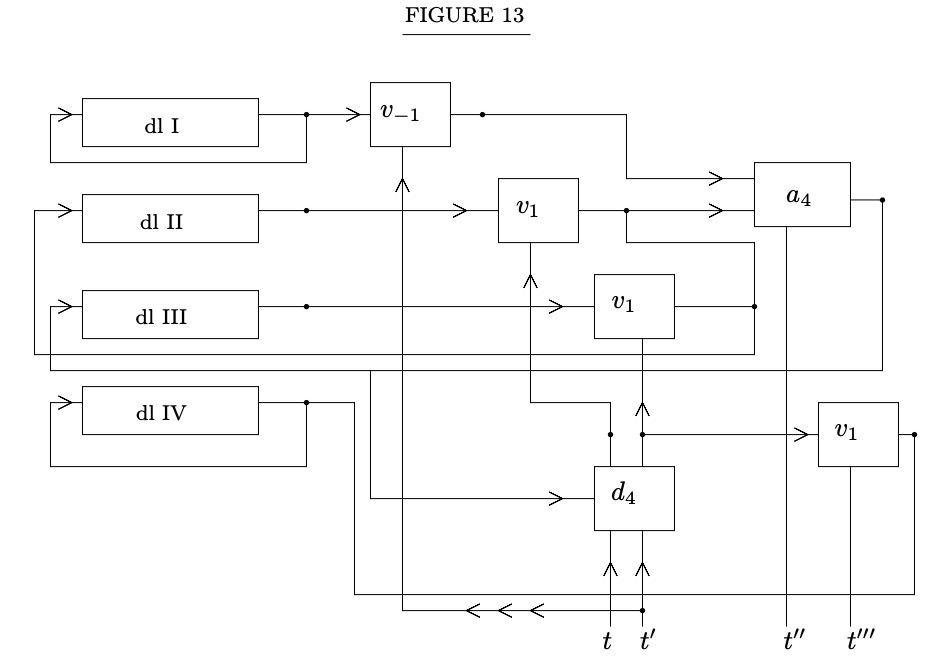
\includegraphics[width=\textwidth]{./pics/12.jpeg}
\caption{除法器}
\end{figure}

\subsection{THE BINARY POINT}

二进制点和符号对加减法影响甚微,而对乘除则关系颇大。一个问题
是,我们需要截取乘法的结果至原来的一半——我们需要通过积的
二进制点的位置决定省去哪部分数。受限于乘法的操作,我们需要处理
乘法小数点的各种情况。经过分析的结果是,二进制点总是紧跟在符号
数字之后,可以保证每次乘法都能够进行,并且小数点具有固定
的位置。而这要求计算过程中所有数字在-1和1之间——即,要求数字需要
可以被移位运算,且需要加法器引入一些诸如结果范围的要求,然后通过一些验证
器保障这些。最后,四舍五入器是容易的,只需要超出的位做与运算即可。

\begin{figure}[H]
\centering
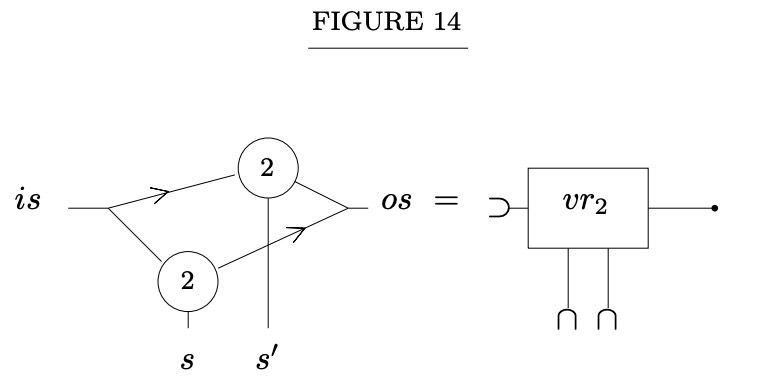
\includegraphics[width=\textwidth]{./pics/13.jpeg}
\caption{舍入器}
\end{figure}

\subsection{CIRCUIT FOR THE ARITHMETICAL OPERATION √ . OTHER OPERATIONS}

求根类似于除法,每次在已计算的结果的基础上判断下一位是1还是0,
因而可以用类似除法的网络完成——区别仅在于要左移两位且需要按计算
结果求出减数——所做的操作不过成二和加一,这是容易实现的。这种
类似性致使开根所面临的(比如小数点上的)问题也与除法类似。

接下来对于上述运算是否需要存在于CA中的问题,+、-毫无疑问需要存在,
而$\times$相对整个系统的复杂性较为简单,且可以配合加法,而且
性能优于维护表,因而存在也是合理的。对于$\div$和$\sqrt{}$,尽管
可以通过函数表或者乘法的迭代收敛完成,但这个代价会是巨量的表
或者巨量的乘法。这是在真空管器件上(乘法不并行)不能接受的。因而
$\div$和$\sqrt{}$最好也放入CA中。这些构建好的网络只需要加上选择
器即可得到具有所有运算功能的模块。

另一个问题是,CA中需要包含其他的运算吗?答案是不。其他运算并
不像除法和开根一样可以用耗时很短的、硬件开销不大的电路完成
,但可以使用插值的方式通过乘法完成。因而,CA中不再包含其他的运算
是合适的。

\begin{figure}[H]
\centering
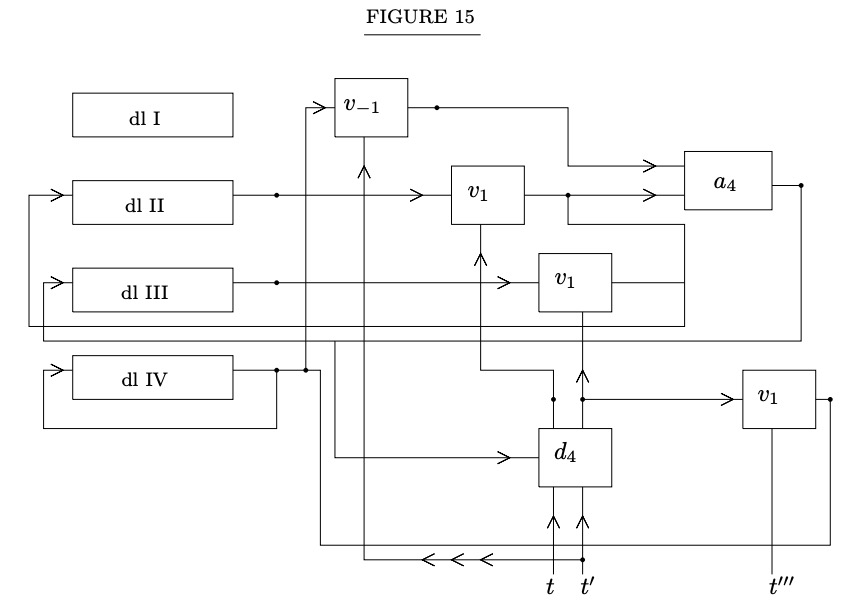
\includegraphics[width=\textwidth]{./pics/14.jpeg}
\caption{求根器}
\end{figure}

\subsection{ORGANIZATION OF CA. COMPLETE LIST OF OPERATIONS}

接下来我们考察如何完成M和CA之间的交互。首先,
要实现上述5种计算,梳理一下会发现CA需要2个输入($I_{ca}, J_{ca}$)和1个输出($O_{ca}$)。
因而,M需要能够和$I_{ca}$、$J_{ca}$、$O_{ca}$交互。
但是是否M的每个部分都需要连接$I_{ca}$、$J_{ca}$,CA作中
转站时从M的一部分到另一部分到传输又应该怎么处理呢?

按照以时间次序避免并行的想法,第一个问题可以通过第一个参数先输入
到$I_{ca}$再从$I_{ca}$输入到$J_{ca}$完成,所以不需要都连接。

对于第二个问题,尽管可以通过+0完成M输入到$I_{ca}$到$O_{ca}$再到
M的过程,但这个仍可以得到优化。文中建议新增i,j两个操作分别直接
将$I_{ca}$、$J_{ca}$引入$O_{ca}$,这样一是省去了不必要的开销,
另外还可以支持诸如把$O_{ca}$引入$I_{ca}J_{ca}$的操作以完成
翻倍、乘方、倒数、相反数等系列操作。这是很重要的。

之后,我们需要在给定的方案中进行选择的能力,即在IJ中选择的能力。
我们决定添加s:效果类似于$return\ (x\geq y)?u:v$,做法是
在一个时钟周期内运算x-y,下一个周期拿到符号读入u,v然后再进行
i操作或j操作。类似的构架也可以将x,y视为单一的x进行选择。

最后,我们需要db,bd两个二进制-十进制转换的操作。

\begin{figure}[H]
\centering
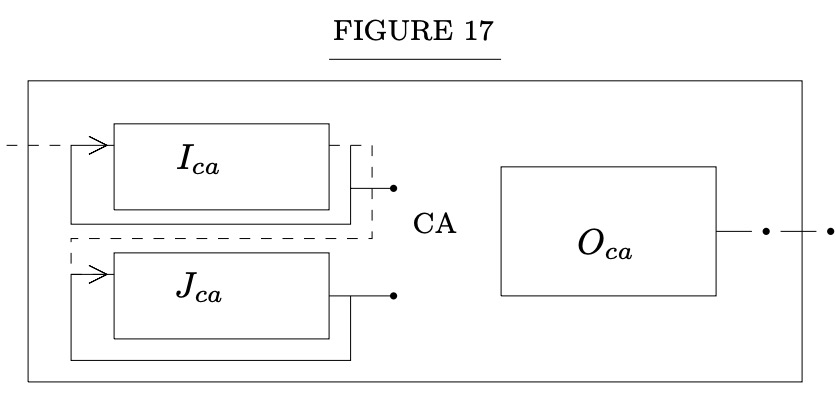
\includegraphics[width=\textwidth]{./pics/15.jpeg}
\caption{CA的输入输出}
\end{figure}

\subsection{CAPACITY OF THE MEMORY M. GENERAL PRINCIPLES}

虽然之前考虑过内存,但是使用的$dl(k)$不过是一种延迟而已。内存
绝对不是这种循环(或延迟)类型的必要条件。我们需要考察其他类型。

为刻画M,我们定义内存的容量是存储2进制数字的能力,并且我们把
数字定位32位一个,并将整个内存细分:首先分到单元,然后再将
单元32个一组划分出来成为一个小周期——这简化了内存的组织和设备
的各种同步问题。此外,我们也需要精确到以一个小周期为操作单位的指令组。

对具体模块的内容需求,“指令”需要制定典型问题后确定;常见的函数
表从切换问题的角度和精度的角度有需求限制,两方面的具体分析可以
得到相应的内存大小;初始边界条件有些直接给出不必记住,剩下的
所占内存不会超过中间量;中间量的大小受问题影响,文中的问题分析
需要的变量数,结果位20万单位足够;而统计问题是多方面的,很难作系统
的计划。

文中还剖析了穿孔纸带引发的存储问题。

综合问题的出现状态,最终结果是需要一个容量约25万单位的存储器M。这对
当时来说构成了计算机的主要瓶颈。为达到这个数字,M的dl需要选择更特殊
结构的线性电路——这种物理器件的存在性使M的制造成为可能。

然而,上述物理器件也存在着对于容量大小的限制,并且需要做到容量
尽可能大以达到减少器件数的效果。同样我们可以将多个dl输入输出相连
配以SG(用以观察信息和控制输入输出)等器械解决这个问题。而SG的数目和
性能的要求也在文中作了更涉及底层的进一步分析,其配置需要从平衡设备
各种操作的时间要求的一般原则中得到。

由于一般运算会进行插值,每个从M中读取的元素一般会进行至少2次乘法,
因而花时间从M中读数是可以接受的。通过乘法的时间就能根据分析
反配出之前提到的SG的参数。总的来说,这是器件性能和器件数量之间
的权衡。

虽然也有其他物理器件的选择,但是他们当时的种种缺陷使得现阶段
选择的物理器件被最后选定。

\begin{figure}[H]
\centering
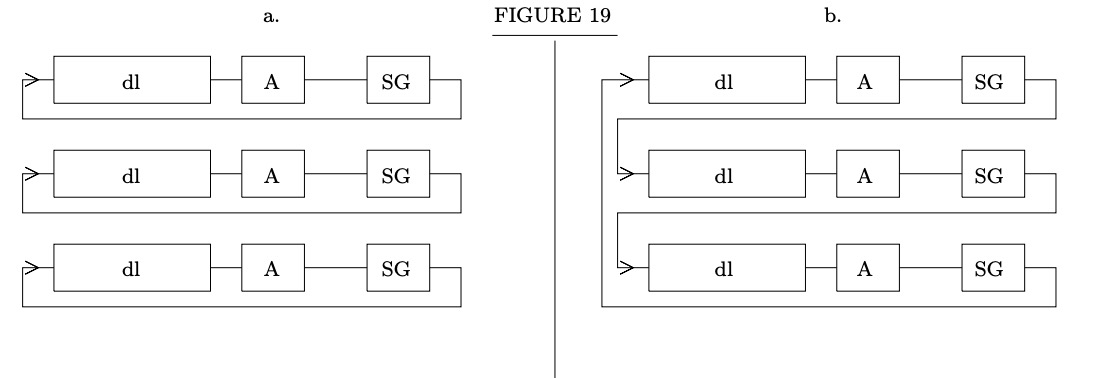
\includegraphics[width=\textwidth]{./pics/16.jpeg}
\caption{dl与存储}
\end{figure}

\subsection{ORGANIZATION OF M}

SG是一个开关和门控机构,我们希望在E-ELEMENTS的角度构建它。
然而A仅仅是恢复脉冲,没有必要这么讨论。

dl需要从向有需求的元件发送和接受信号,因而需要输入输出信号的
线路$L_i, L_o$,我们的元件需要在合适的情况下选择合适的线路。
并且,当不需要传播的时候它的信号应该通过另一条线传入下一个dl。
由于每时刻C只有一个补充链接链接SG,因而控制逻辑放在此处是合适的。
以这个目标为指引,在对延迟等信息仔细考量之后,我们便能得到相应元件
的初步草图了。

\begin{figure}[H]
\centering
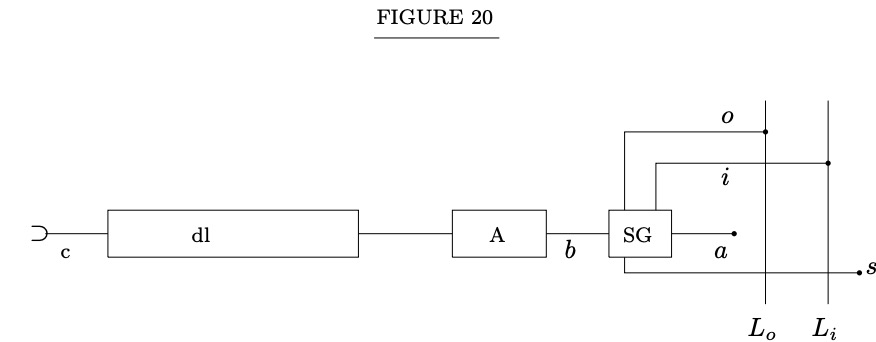
\includegraphics[width=\textwidth]{./pics/17.jpeg}
\caption{A与SG}
\end{figure}

\subsection{CC AND M}

接下来,我们希望给控制器提供代码和对应的操作。这些代码存在M里。
代码分为4类:运算、转移内存内容、指令转移、控制IO。
只考虑第2,3种:M之间的转移
可以通过CA完成,CA内部的转移很容易完成,因而只需考虑CA与M之间
的转移,这在上一章已经涉及了。
判断下一条指令通常是按序选取下一条,并附带了类似jmp的
指令。这里需要处理一下周期内等待指令的小细节,使用类似的
与M的交互手段也可以完成。由于瞬态转移
总能被永久转移替代,因而文中抛弃了瞬态转移。当然,由于在顺序的
指令中CA也需要和M相连,短暂地暂存现有的位置和抛弃链接是必要的。

值得一提的是,在这里,在等待时间、循环分割的诸多细节方面也有
很多扩展的空间。

\subsection{THE CODE}

下一步,我们根据上一节的操作制定相应的代码。指令在文中同样
也是小循环。文中使用了第一位来标识小循环是标准数还是指令。
指令按上述四种要求划分(最终可以划分出8种指令)。
运算指令通过4bit指定10种运算之一,
其运算数通过先I后J的方式输入。这里有一些细节:有时运算的结果
是否被清出$O_{ca}$是值得商榷的,因而需要流出1bit指定是否
清除之。对每个操作数也应该分配相应的空间。数字转移指令等同类的
指令也是类似的划分方式。类似我们可以得到其他指令的格式。尽管
有些指令较短,把他们放到一个小循环里可以节省空间,
但不合适的合并会导致诸多问题,譬如:同时运行多个函数
,这是本文认为不好的;打乱了操作时间;不会太优化
性能;同时,保留一些可以被扩展的位也是必要的。所以
文中在权衡后给出了一些可以允许的组合。在这个准则下,按照对应
位置对应操作数即可设计出最终我们需要的代码。

\section{冯诺伊曼结构特点分析}

\subsection{将计算机划分为五个基本模块}

冯诺伊曼结构将计算机划分为5个主要部分,以将复杂的计算机系统
分而治之。尽管5部分之间仍有千丝万缕的关系,但每部分的功能
被干净地独立了出来。这使得每一部分的功能设计目标更加清晰且
只需提供相应的借口就可以相对独立地考察之。功能优化也可以注重
于一点讨论。

\subsection{以神经元的视角观察元件组成}

冯诺伊曼将1bit的存储器类比为人类的神经元这一具有“维持刺激状
态、不以损失能量的形式传递信号”能力的、具有“唯一突触延时”的
、不必过于深入考究细节的概念化元件,很好地给上层跟下层构架划
清了界限,并且跟现实世界的相合性保证了下一步设计的安全性、抽象
概念的整洁性保证了之后的设计只需要从逻辑角度出发,方便了之后的
设计。

\subsection{使用二进制,而非十进制}

冯诺伊曼架构考察了硬件的特性,指出了两个平衡态的元件是方便、安全且
容易实现的,进而指明了二进制和计算系统的相合性。同时,为与人类
的认知相合,冯诺伊曼架构将10进制保存在了R和IO设备中,方便了人类
的操作控制。

\subsection{程序作为M的一部分存储}

冯诺伊曼架构将程序编码以二进制形式存储在M中,使得CC可以自动解析
命令执行程序,节省了人为控制程序的缓慢步骤,加快了程序运行,并将
软硬件分割开来,使得软硬件能够在一套公有的协议下、不顾及另一面地自由地协同发展。

\subsection{面向具体问题的微体系架构设计}

冯诺伊曼的具体设计,譬如内存大小和系统设计面向的性能要求都是基于
具体问题而来的。譬如,一般函数的泰勒展开精度在2-4项即可达到要求,
因而,从内存读数的时间被要求在不会影响两次乘法的时间内。又,内存
具体大小的设计是根据一个具体问题一般所需要的具体参数个数确定。

\section{当前计算设备分析对比}

我们选择m1芯片与冯诺伊曼提出的最初的架构进行对比。笔者希望注重对比处理器和存储
两个部分。

\subsection{C}

在M1芯片中,C的部分由多种处理器构成,而非文中所述的一种。CPU,GPU,NPU等多种
处理器协调完成对数据和指令的处理功能。每种处理器也并非单一的一块,而是由多块
并行使用以加速任务——这明显与冯诺伊曼尽力回避“并行”的想法相异。

另外,不同于冯诺伊曼把“不冲突”的指令合在一个“小周期”中以尽量加速指令,苹果的M1
使用了ARMv8-A 指令集,每条指令长度固定,不会出现多条指令挤占同一内存单元的现象,
并通过乱序执行技术来完成同一时间尽量执行多条指令的目标。

在乘法和浮点数计算部分,浮点数流水线、浮点重命名寄存器等设计使得M1的运算性能远高于
设计粗糙的冯诺伊曼原稿。

\section{M\&R}

M1的芯片中具有巨量的晶体管构成内存。与冯诺伊曼原始手稿中的M、R两层不同的是,M1芯片
中罗列了多级的高速缓存,芯片的成本逐级递增,而其性能亦然;另有,R并非使用了十进制,
这里一般均使用二进制存储,只在输出端或必要时使用十进制。

另外M1芯片的访存也比原始手稿中复杂许多,M1芯片将所有硬件模块的内存地址统一以避免多处理器
访问内存时的额外转移,这就需要极其繁琐的处理过程,不是简单的A和SG可以完成的。

\section{“非冯结构”调研分析}

\subsection{哈佛架构}

哈佛结构将程序存储器与数据存储器分离,两部分通过不同的总线与
存储器进行交互。cpu的运转变为先从程序存储器中读取程序,然后再
从数据存储器中读取相应的数据。

\paragraph*{主要种类}

AVR、ARM9、ARM10、ARM11等

\paragraph*{优点}

\begin{enumerate}
    \item 独立的程序存储结构和数据存储结构使指令长度不受限于数据长度,两者长度可以更为自由地安排。
    \item 分离的程序读取和数据读取可以使得读取程序操作不受限于数据的读取,减少取址和取数的冲突,提高流水线式读取、解析程序的效率。
\end{enumerate}

\paragraph*{缺点}

\begin{enumerate}
    \item 分离的总线会导致总线的相对宽度降低,数据传输的效率会降低。
    \item 多个地址空间很可能带来操作的不便。
\end{enumerate}

\begin{figure}[H]
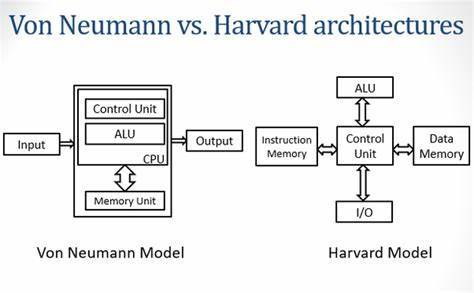
\includegraphics[width=\textwidth]{./pics/18.jpg}
\caption{哈佛架构和冯诺依曼架构}
\end{figure}

\subsection{神经网络}

神经网络试图模仿生物脑部神经,通过元件模拟神经元的互联以构建用于计算
的网络系统。

\paragraph*{主要种类}

循环神经网络、卷积神经网络、前馈神经网络等

\paragraph*{优点}

\begin{enumerate}
    \item 可以实现类似生物的自学习能力和自适应能力。
\end{enumerate}

\paragraph*{缺点}

\begin{enumerate}
    \item 需要巨量的数据和计算资源。
    \item 神经网络框架需要良好的参数才能获取良好的效果。
\end{enumerate}

\begin{figure}[H]
\centering
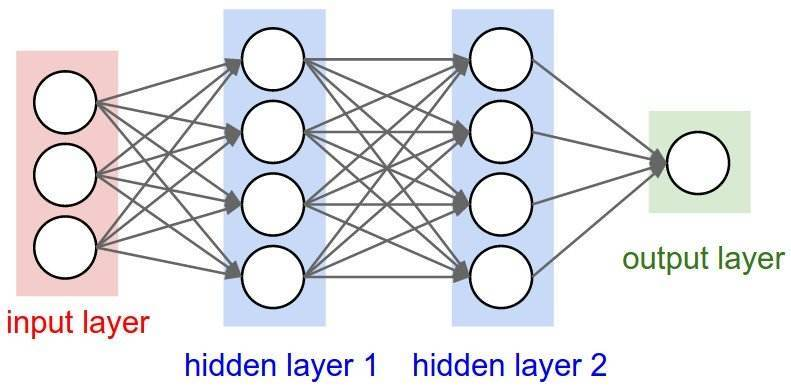
\includegraphics[width=.8\textwidth]{./pics/7.jpg}
\caption{神经网络}
\end{figure}

\subsection{图灵机}

图灵机是从理论上定义“计算”的计算模型。一台图灵机只由无限长
的纸袋、读写头、状态及转移函数组成。他根据读取到的信息和状态
进行前进、后退或不动的操作,并转移现在的状态,直至纸带标识
图灵机终止。

\paragraph*{主要种类}

图灵机并未真正被实现过,没有主要种类之分。

\paragraph*{优点}

\begin{enumerate}
    \item 由于任意算法都对应一种图灵机,因而图灵机具有计算完备性。
\end{enumerate}

\paragraph*{缺点}

\begin{enumerate}
    \item 图灵机在现实中不太好实现,现在仍没有真正实现投入使用的图灵机。
\end{enumerate}

\begin{figure}[H]
\centering
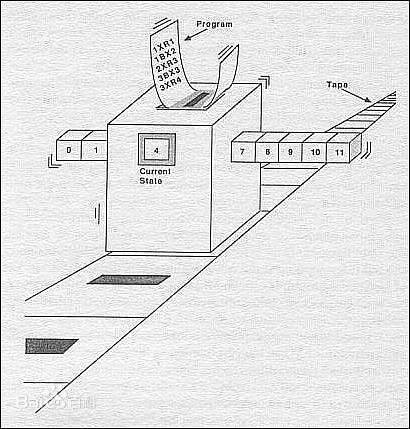
\includegraphics[width=.6\textwidth]{./pics/8.jpg}
\caption{图灵机}
\end{figure}

\subsection{数据流计算机}

数据流计算机是以数据流为主要视角、依据数据是否可用决定是否
触发指令的体系架构。

\paragraph*{主要种类}

静态数据流机、动态数据流机

\paragraph*{优点}

\begin{enumerate}
    \item 可以在又需求的时候才使用运算资源,对运算资源进行高效利用。
    \item 不以指令流方式运转,省去对指令读取和解析所耗费的时间,更容易实现高度并行。
\end{enumerate}

\paragraph*{缺点}

\begin{enumerate}
    \item 没有冯诺伊曼架构中固定的指令、存储器结构,需要在特定场景设计特定数据流计算机。
\end{enumerate}

\section{参考文献列表}

\begin{enumerate}
    \item 个人图书馆:《深度解读苹果M1芯片》$\\http://www.360doc.com/content/22/0504/18/78456304\_1029734816.shtml$
    \item CSDN:《哈佛架构和冯诺依曼架构》$\\https://blog.csdn.net/m0\_74377037/article/details/127657089$。
    \item CSDN:《哈佛结构和冯诺依曼结构特点》$\\https://blog.csdn.net/m0_52561981/article/details/122798969$。
    \item EEPW:《哈佛架构》$\\http://www.eepw.com.cn/article/201608/295773.htm$
    \item 百度百科:《数据流计算机》$\\https://baike.baidu.com/item/\%E6\%95\%B0\%E6\%8D\%AE\%E6\\\%B5\%81\%E8\%AE\%A1\%E7\%AE\%97\%E6\%9C\%BA/10778431?fr=aladdin$
\end{enumerate}

\end{document}